\subsection{Brief Review of NGCF, LightGCN and GCF}\label{subsubsec:brief-review}
Neural Graph Collaborative Filtering (NGCF) was published in 2019, and was a state of the art method, that utilized graph convolutional networks (GCN) for collaborative filtering \cite{NGCF_2019}.
GCN was originally proposed for node classification where each node has rich attributes, but for collaborative filtering the nodes only contain node IDs \cite{lightgcn,kipf2017semisupervised,NGCF_2019}.
This is something that LightGCN took advantage of and simplified NGCF by removing the nonlinear activation function and the feature transformation, which showed promising results in their experiments.
Later Meng Liu et. al then created a method called BiTGCF which utilized GCN and transfer learning between two domains \cite{BiTGCF}.
They also added GCF which is a degenerate version of BiTGCF that does not utilize transfer learning between two domains, but is a single domain method such as LightGCN and NGCF.
BiTGCF and GCF removes the features transformation and nonlinear activation function of NGCF, which was inspired by LightGCN, but chooses to keep different aspect of NGCF.
In their experiments Meng Liu et. al showed that both GCF and BiTGCF showed large improvements over both LightGCN and NGCF, but BiTGCF only showed smaller improvements over GCF, which can indicate that high connectivity caused by GCN has larger effect on recommendation than transfer learning between other domains.
In this paper we only concentrate on single domain methods, and therefore will only focus on GCF of these two methods.

\subsubsection{Graph Convolutional Networks}
GCN for collaborative filtering can generally be abstracted as \cite{BiTGCF}
\begin{equation}
    e_u^{(k+1)} = AGG(e_u^{(k)},e_i^{(k)} : i \in \mathcal{N}_u),
\end{equation}
where $AGG(\cdot)$ is an aggregation function, and $e_i^{(k)}$ and $e_u^{(k)}$ denotes the embeddings for user $u$ and item $i$ after $k$ propagation layers.
The embedding propagation for items can be obtained similarly as the embeddings with users by replacing $u$ with $i$ and vice versa.
$\mathcal{N}_u$ and $\mathcal{N}_i$ denotes the one hop neighbors from user $u$ and item $i$ respectively \cite{lightgcn,BiTGCF,NGCF_2019}.\\
On \autoref{fig:gcn-figure} a generalized figure of LightGCN, GCF and NGCF can be seen.
Graph convolutions are conducted on the initial embeddings, where an embedding function is used.
The graph convolutions are illustrated on \autoref{fig:gcn-convolutions} and this figure shows how the signal from $e_{i_1}^{(0)}$ passes through $e_{u_3}^{(1)}$ and $e_{i_4}^{(2)}$ to $e_{u_1}^{(3)}$.
This is how the graph convolutions are performed on all users and items.
When the convolutions have been conducted on each layer, it is given as input to the layer combination, which could either be concatenation or weighted summation.
An example can be seen on \autoref{fig:layer-combination}, where each array symbolizes a layer.
\begin{figure*}[h!]
    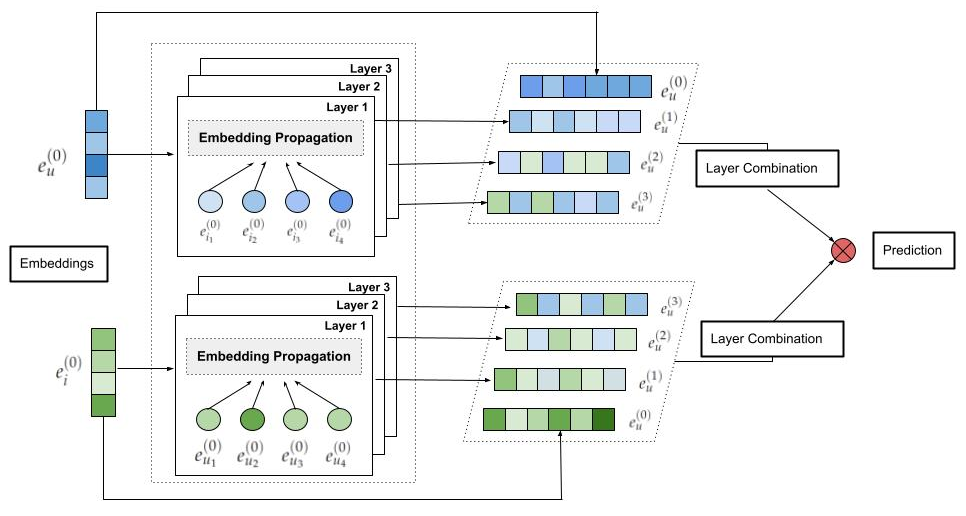
\includegraphics[width=1.1\textwidth]{figures/generalized-gcn-figure.PNG}
    \centering
    \caption{Generalized structure of NGCF, LightGCN and GCF}
    \label{fig:gcn-figure}
\end{figure*}
\begin{figure}[h!]
    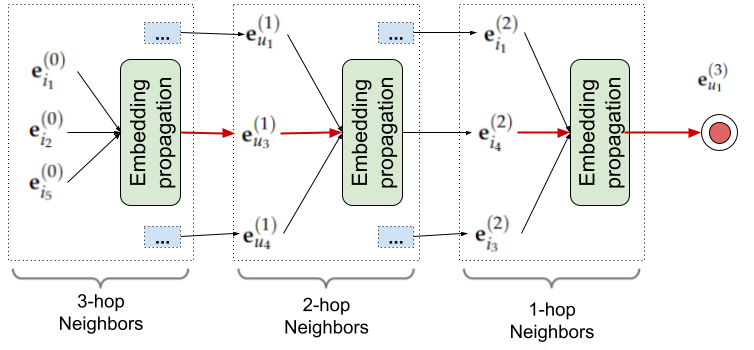
\includegraphics[width=0.5\textwidth]{figures/embedding-convolutions.png}
    \centering
    \caption{Illustration of three graph convolutions for $u_1$}
    \label{fig:gcn-convolutions}
\end{figure}
\begin{figure}[h!]
    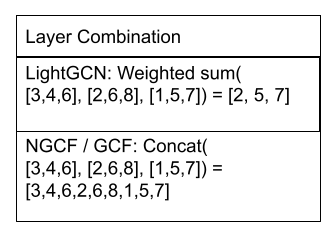
\includegraphics[width=0.4\textwidth]{figures/layer-combination.png}
    \centering
    \caption{Example of weighted summation and concatenation as layer combinations.}
    \label{fig:layer-combination}
\end{figure}
Following this section we will describe the embedding propagation for users and the final layer combination for NGCF, LightGCN and GCF.

\subsubsection{Embedding Propagation in NGCF:}
The embedding propagation in NGCF is defined as,
\begin{equation}
    \mathbf{e}_{u}^{(k+1)} = \mbox{LeakyReLU}(\mathbf{m}^{(k)}_{u \leftarrow u} + \sum^{}_{i \in \mathcal{N}_u} \mathbf{m}^{(k)}_{u \leftarrow i}),
    \label{eq:ngcf-embedding-propagation}
\end{equation}
where LeakyReLU is the nonlinear activation function, $\mathbf{m}^{(k)}_{u \leftarrow i}$ is the message construction from users u to item i, and $\mathbf{m}^{(k)}_{u \leftarrow u}$ is the self connection.
These are respectively defined in \autoref{eq:message-construction-i-to-u} and \autoref{eq:self-connection} \cite{NGCF_2019}.
\begin{equation}
    \mathbf{m}^{(k)}_{u \leftarrow i} = \frac{1}{\sqrt{|\mathcal{N}_u||\mathcal{N}_i|}}(\mathbf{W}^{(k)}_1\mathbf{e}^{(k)}_i + \mathbf{W}^{(k)}_2(\mathbf{e}^{(k)}_i \odot \mathbf{e}^{(k)}_u)),
    \label{eq:message-construction-i-to-u}
\end{equation}
\begin{equation}
    \mathbf{m}^{(k)}_{u \leftarrow u} = \mathbf{W}_1^{(k)}\mathbf{e}_u^{(k)}
    \label{eq:self-connection}
\end{equation}
For \autoref{eq:message-construction-i-to-u} and \autoref{eq:self-connection} $W_1$ and $W_2$ are the trainable weight matrices used to perform feature transformation at each layer.
$\frac{1}{\sqrt{|\mathcal{N}_u||\mathcal{N}_i|}}$ is the graph Laplacian norm used to normalize the embeddings.
The final embedding is calculated by concatenating each embedding layer as seen on \autoref{eq:ngcf-concat-embed} \cite{NGCF_2019}.
\begin{equation}
    \mathbf{e}_u = \mathbf{e}_u^{(0)}||...||\mathbf{e}_u^{(k)}
    \label{eq:ngcf-concat-embed}
\end{equation}

\subsubsection{Embedding Propagation in LightGCN}\label{subsubsec:LightGCN-embed-propagation}
The embedding propagation for LightGCN is defined as \cite{lightgcn},
\begin{equation}
    \mathbf{e}_{u}^{(k+1)} = \sum^{}_{i \in \mathcal{N}_u} \frac{1}{\sqrt{|\mathcal{N}_u||\mathcal{N}_i|}} \mathbf{e}_i^{(k)}
\end{equation}
As can be seen, LightGCN simplified NGCF by removing the activation function, transformation matrices, the self loop and the inner product between the user and item embeddings.
Additionally LightGCN changes the layer combination from concatenation to weighted summation as shown here:
\begin{equation}
    \mathbf{e}_u = \sum_{k=0}^{K} \alpha_k \mathbf{e}_u^{(k)},
    \label{eq:lightgcn-sum}
\end{equation}
where $K$ is the total number of layers and $\alpha_k$ is a hyper parameter used to denote the importance of the $k$-th embedding \cite{lightgcn}.
$\alpha_k$ is set to $1 /(K + 1)$ for simplicity.

\subsubsection{Embedding Propagation in GCF}\label{subsubsec:GCF-embed-propagation}
The embedding propagation in GCF is defined as \cite{BiTGCF},
\begin{equation}
    \mathbf{e}_{u}^{(k+1)} = \mathbf{e}_{u}^{(k)} + \sum^{}_{i \in \mathcal{N}_u}  \frac{1}{\sqrt{|\mathcal{N}_u||\mathcal{N}_i|}}\left( \mathbf{e}_i^{(k)} + \mathbf{e}_i^{(k)} \odot \mathbf{e}_u^{(k)} \right)
    \label{eq:GCF-embedding}
\end{equation}
As can be seen GCF adds the self connections and the inner product between the users and items compared to LightGCN.
The purpose of the inner product is that the more the user and item nodes have in common the greater the value will be passed to the center node \cite{BiTGCF}.
Self connection is used to retain the information of the original node.
Additionally GCF uses concatenation as layer combination, which was also used by NGCF in equation \autoref{eq:ngcf-concat-embed}.
